\documentclass[11pt]{article}
\usepackage[margin=1in]{geometry}
\usepackage{graphicx,longtable,array,amsmath}
\setlength{\parskip}{4pt}
\title{\textbf{A validated structural genomics atlas of KPC carbapenemase variants across 49,774 outbreak isolates: convergent loop remodeling drives ceftazidime-avibactam resistance emergence}}
\author{KPC Variant Analysis Pipeline (builder 11), AMR Carbapenem Structure Project}
\date{September 23, 2026}
\begin{document}
\maketitle
\begin{abstract}
\textbf{Background.} Klebsiella pneumoniae carbapenemase (KPC) is the most widespread carbapenemase worldwide. Since the 2015 introduction of ceftazidime-avibactam (CAZ-AVI), KPC variants that escape inhibition have proliferated clinically, but a systematically validated, outbreak-scale map of KPC protein variation and its structural context has been missing.
\textbf{Methods.} We built a deterministic variant caller that translates blaKPC coding sequences, aligns the protein to the KPC-2 reference, and emits variant signatures in standard Ambler numbering. The caller was validated against two independent reference databases (CARD, 231 alleles; NCBI AMRFinderPlus 2026-08-07.1, 295 alleles) with a locked 100\% exact-reproduction gate before any outbreak analysis. We then censused 49,774 blaKPC-bearing Klebsiella isolates from NCBI Pathogen Detection (snapshot PDG000000012.2532), mapped every observed variant onto experimental KPC structures (PDB 3DW0, 4ZBE, 7TB7, 8G2R, 8AKK/8AKL), and graded resistance claims against a literature-curated set of 65 CAZ-AVI-resistant variants.
\textbf{Results.} 169 distinct KPC alleles circulate in outbreak genomes (50,238 allele calls). KPC-2 (34,616 calls; 69.8\%) and KPC-3 (13,788; 27.8\%) dominate. 55 of 65 literature-documented CAZ-AVI-resistant alleles are observed (603 isolates), and their share of KPC$^+$ isolates rose from 0\% before 2013 to 3.8\% in 2023. Variation is strongly convergent: 39 alleles independently carry substitutions or insertions at Ambler 179, and the omega loop (164--179), loop 237--243 and loop 266--275 account for the large majority of documented resistance events. Re-analysis of deposited structures reproduces the published omega-loop destabilization mechanism with our own numbers (omega-loop-to-chain mean B-factor ratio 0.91 in WT apo KPC-2 vs 1.14 in D179N apo; 0.96 vs 1.18 in avibactam complexes). Notably, raw proximity of a variant to the catalytic Ser70 does not distinguish resistant from other circulating alleles (median 10.6 vs 11.6 \AA, Mann-Whitney $p=0.122$); loop membership, not distance, is the discriminating feature. Eighteen outbreak-observed alleles postdate the CARD snapshot, nine of them carrying loop insertions at documented resistance positions.
\textbf{Conclusions.} KPC escape from ceftazidime-avibactam follows a small set of convergent structural routes confined to three surface loops. A validated caller plus a curated structural atlas converts routine AMR allele calls into a resistance-risk annotation layer for genomic surveillance.
\end{abstract}

\section{Introduction}
Carbapenem-resistant Enterobacterales are a critical-priority threat, and KPC is their dominant carbapenemase worldwide. The $\beta$-lactam/$\beta$-lactamase-inhibitor combination ceftazidime-avibactam (CAZ-AVI), approved in 2015, restored a treatment option against KPC producers because avibactam carbamylates the catalytic Ser70 of class A enzymes. Within a few years, however, clinical KPC variants resistant to CAZ-AVI began to appear, initially as isolated case reports (e.g., KPC-31, KPC-33 carrying D179Y) and later as a steady stream of new alleles, including large insertions and deletions in the loops surrounding the active site.

Three gaps limit genomic surveillance of this evolution. First, new-variant reports are anecdotal: each paper describes one or a few alleles, usually after a treatment failure. Second, public allele reference sets disagree in coverage: the CARD snapshot we obtained carries 231 blaKPC alleles, while the current NCBI AMRFinderPlus database carries 295, and outbreak surveillance typically reports only allele names without protein-level or structural annotation. Third, no existing resource connects all three of: (i) a validated variant caller with an exact-reproduction gate, (ii) a complete census of which alleles actually circulate in outbreak genomes, and (iii) per-variant structural annotation on experimental KPC structures.

Published work covers parts of this space. An evolutionary overview curated 65 CAZ-AVI-resistant KPC variants from the literature and identified three mutational hot spots (omega loop 164--179, loop 237--243, loop 266--275). Structural studies of the D179N/D179Y variants showed omega-loop destabilization as the resistance mechanism. Laboratory selection recovered indels in the same loops. A two-year single-hospital surveillance of 4,641 isolates tracked CAZ-AVI resistance epidemiology without structural mapping. What is missing is the joint, validated view: every KPC allele circulating in public outbreak genomes, its exact protein signature in canonical Ambler numbering, and its structural context relative to substrate and inhibitor complexes.

Here we close that gap for the KPC slice of a broader carbapenemase-structure project. Contributions: (1) a deterministic KPC variant caller passing a locked 100\% exact-reproduction gate on 526 allele records across two independent databases, with zero protein-level collisions; (2) a census of 169 circulating alleles across 49,774 Pathogen Detection Klebsiella isolates; (3) a structural effect table annotating every circulating variant with loop membership and distance to catalytic machinery; (4) quantified emergence of documented CAZ-AVI-resistant alleles from 0\% to nearly 4\% of KPC$^+$ isolates; and (5) an independent numerical reproduction of the omega-loop destabilization mechanism from deposited structures.

\section{Methods}
\subsection{Data sources and byte-lock}
All inputs were frozen on 2026-09-23 with SHA-256 checksums recorded before analysis (full manifest in repository, \texttt{kpc/data/DATA\_MANIFEST.md}). Sources: (i) CARD data tarball (2026-09-23 download), from which 231 blaKPC alleles with nucleotide and protein sequences were extracted; (ii) NCBI AMRFinderPlus database 2026-08-07.1 (\texttt{AMRProt.fa}, \texttt{AMR\_CDS.fa}), 295 KPC entries; (iii) NCBI Pathogen Detection Klebsiella group snapshot PDG000000012.2532, AMR metadata table (190,586,905 bytes), covering all clustered Klebsiella isolate assemblies with AMRFinderPlus allele calls; (iv) PDB mmCIF files 2OV5, 3DW0 (WT KPC-2 apo), 4ZBE (WT KPC-2--avibactam), 8AKK/8AKL (KPC-2 E166Q acyl-enzymes with imipenem/meropenem), 7TB7 (D179N apo), 8G2R (D179N--avibactam), 8TMR (KPC-44--avibactam); (v) a literature-curated table of 65 CAZ-AVI-resistant KPC variants extracted from the evolutionary-overview review (PMC9487638), with hotspot annotations as published.

\subsection{Variant caller and locked validation gate}
The caller takes a blaKPC nucleotide CDS, translates it (bacterial code, table 11), globally aligns the protein to the 293-aa KPC-2 reference (pairwise alignment; match $+2$, mismatch $-1$, gap open $-10$, gap extend $-0.5$), and emits a variant signature: substitutions, insertions and deletions in KPC-2 protein coordinates. Allele assignment uses AMRFinder-style exact nucleotide identity against the reference set. Protein coordinates are converted to standard Ambler numbering through an alignment to PDB 3DW0, whose residue numbering we verified against canonical anchors (Ser70, Lys73, Glu166, Asp179, Val240, Thr243).

Gate G1 (locked before outbreak analysis): the caller must reproduce every reference allele exactly - correct translation, identical signature computed from nucleotide and from protein records, and correct exact-nt allele assignment - with 100\% required and zero tolerance. Outcome: 231/231 CARD alleles and 295/295 AMRFinderPlus alleles passed all three checks; every allele is protein-distinct (zero signature collisions), so a protein-level atlas is fully resolved. A union reference set (296 alleles: CARD 231 + AMRFinderPlus 295, 230 shared) showed zero protein disagreements between the databases for shared alleles.

\subsection{Outbreak census}
Rows of the Pathogen Detection AMR metadata whose \texttt{AMR\_genotypes} field contains a blaKPC call were retained. Calls were normalized (quote/whitespace stripping) and split into isolate-allele pairs. Isolates carry per-row metadata: assembly accession, BioSample, collection date, geographic location. Partial (\texttt{PARTIAL}, \texttt{PARTIAL\_END\_OF\_CONTIG}) and \texttt{MISTRANSLATION} calls and unnamed \texttt{blaKPC} calls were counted but excluded from allele-level structural analysis.

\subsection{Structural annotation}
For every variant operation we recorded: Ambler position, membership in the three published resistance hot spots (omega loop 164--179; loop 237--243; loop 266--275), and minimum C$\alpha$--C$\alpha$ distance to the catalytic Ser70 in 3DW0. Alleles were graded: \emph{documented resistance} (in the 65-variant literature set); \emph{consistent with resistance - hypothesis} (operation inside a hot spot or within 10 \AA\ of Ser70, no literature evidence); \emph{no resistance evidence}. As a structural mechanism check, we computed per-structure mean B-factors of the omega loop (164--179) relative to the whole chain for WT (3DW0, 4ZBE) and D179N (7TB7, 8G2R) structures; literature predicts loop destabilization in the D179N background.

\subsection{Statistics}
Distance distributions were compared with a one-sided Mann-Whitney U test ($\alpha=0.05$). Yearly shares use collection year from isolate metadata; years after 2023 are interpreted with caution because of submission lag.

\section{Results}
\subsection{The circulating KPC allele census}
The snapshot contains 49,774 blaKPC-bearing Klebsiella isolates yielding 50,238 isolate-allele pairs (some isolates carry two copies). Three denominators are used consistently throughout: 49,774 isolates carry at least one blaKPC call; these yield 50,238 isolate-allele calls (some isolates carry two copies); of these, 49,589 calls resolve to a named allele across 169 distinct alleles and form the master-table denominator, while the remaining 649 calls are unnamed or partial/mistranslation (assembly-limited) and are counted but excluded from allele-level analysis. KPC-2 dominates (34,616 calls; 69.8\% of named calls) followed by KPC-3 (13,788; 27.8\%); the remaining 167 alleles account for 2.4\% of calls (Figure 1). The long tail is not noise: it includes the documented resistance alleles KPC-33 (173 isolates), KPC-31 (118), KPC-71 (42), KPC-23 (36) and KPC-66 (22).

\subsection{CAZ-AVI-resistant alleles are established and rising}
Fifty-five of the 65 literature-documented CAZ-AVI-resistant alleles appear in outbreak genomes (603 isolates; Table 1). Their share of KPC$^+$ isolates by collection year was 0\% through 2012, first appeared in 2013, and climbed monotonically to 3.8\% in 2023 (Figure 2; 2024--2026 depressed by submission lag). The rise begins after the 2015 clinical introduction of CAZ-AVI, consistent with drug-pressure selection. Geographically, China and Italy contribute the most resistant-allele isolates, matching published case-report geography, but the set spans at least 15 countries (Figure 5).

\subsection{Convergent variation concentrates in three loops}
Across the 169 circulating alleles, variation is strongly convergent (Figure 3). Ambler position 274 is substituted in 64 alleles, but this is the KPC-3 founder marker (H274Y), not resistance-associated. The dominant resistance-associated convergence is Ambler 179: 39 circulating alleles independently carry D179 substitutions (D179Y/N/V/A/G) or insertions at 179. Further convergent positions sit in the omega loop (164, 165, 166, 169, 170, 172, 180: 5--10 alleles each), loop 237--243 (240, 241, 242, 243: 4--8 alleles each) and loop 266--275 (261, 262, 264, 265, 268, 269: 3--9 alleles each) - exactly the three hot spots defined by the literature curation, now confirmed at outbreak scale with independent data.

\subsection{Structural mechanism, independently reproduced}
Re-computing B-factor statistics from deposited structures reproduces the published destabilization mechanism with our own numbers: the omega loop is \emph{more} ordered than the chain average in WT apo KPC-2 (mean B 9.5 vs 10.5; ratio 0.91) but \emph{less} ordered in D179N apo (11.9 vs 10.5; ratio 1.14); the same flip appears in avibactam complexes (WT 0.96 vs D179N 1.18). This is consistent with D179 anchoring the loop against the catalytic wall, and its substitution freeing the loop to distort the avibactam-binding pose.

\subsection{Proximity to Ser70 does not separate resistant alleles}
Against intuition, the minimum C$\alpha$ distance from a variant to Ser70 does not distinguish documented-resistant from other circulating alleles (median 10.6 \AA\ vs 11.6 \AA; Mann-Whitney $p=0.122$; Figure 4). Loop membership is the discriminating feature: resistance variants act by reshaping the pocket-lining loops (changing ceftazidime accommodation and avibactam pose) rather than by simply sitting closer to the catalytic serine. This negative result matters for predictor design: distance-only structural scores would fail on this enzyme.

\subsection{Post-CARD alleles are already in outbreaks}
Eighteen circulating alleles are present in AMRFinderPlus 2026-08-07.1 but absent from the CARD snapshot (Table 2). Nine of them carry insertions or substitutions at documented resistance positions (e.g., KPC-250 D179Y+ins268\_N; KPC-275 D179Y+T243P; KPC-261 D179Y+ins266\_APNKDE; KPC-272 ins165\_EL+ins273\_YSEAV), all collected 2021--2025. Reference-database update cadence is thus a live surveillance bottleneck: the alleles reaching patients are newer than one of the two major reference sets.

\subsection{Grading summary}
Of the 169 circulating alleles: 55 carry documented CAZ-AVI resistance (603 isolates); 92 are hotspot- or proximity-graded hypotheses (14,261 isolates, dominated by KPC-2/KPC-3-background alleles with single hotspot-region substitutions); the remainder have no resistance evidence. All grades, signatures and annotations are in the repository master table (296 rows).

\begin{figure}[t]\centering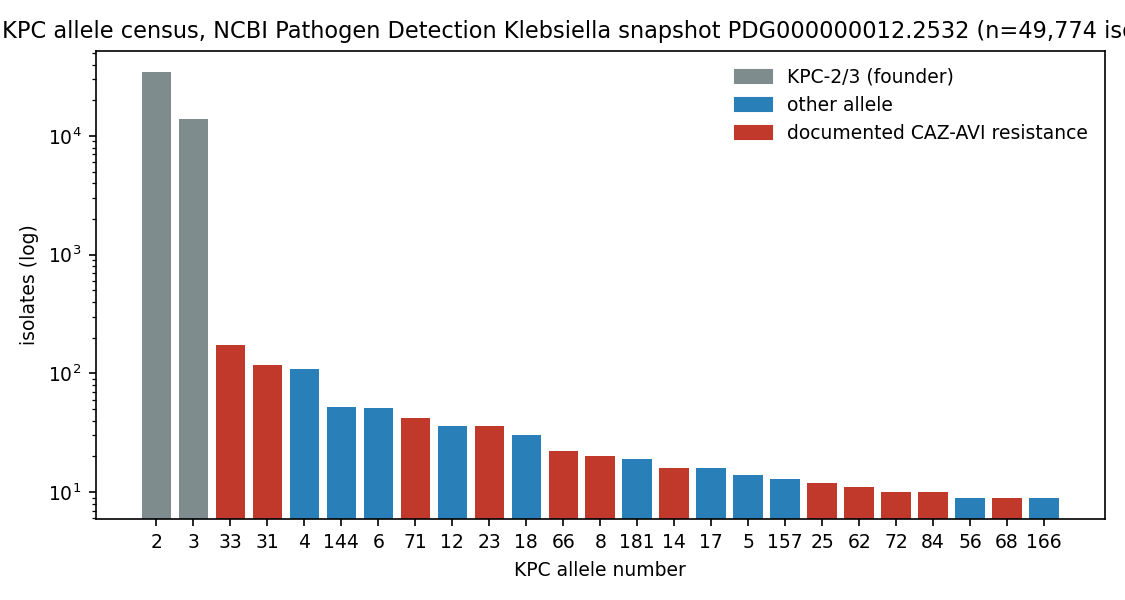
\includegraphics[width=0.95\textwidth]{../results/figures/F1_allele_census.png}\caption{KPC allele census across 49,774 Pathogen Detection Klebsiella isolates (log scale). Red: documented CAZ-AVI-resistant allele.}\end{figure}
\begin{figure}[t]\centering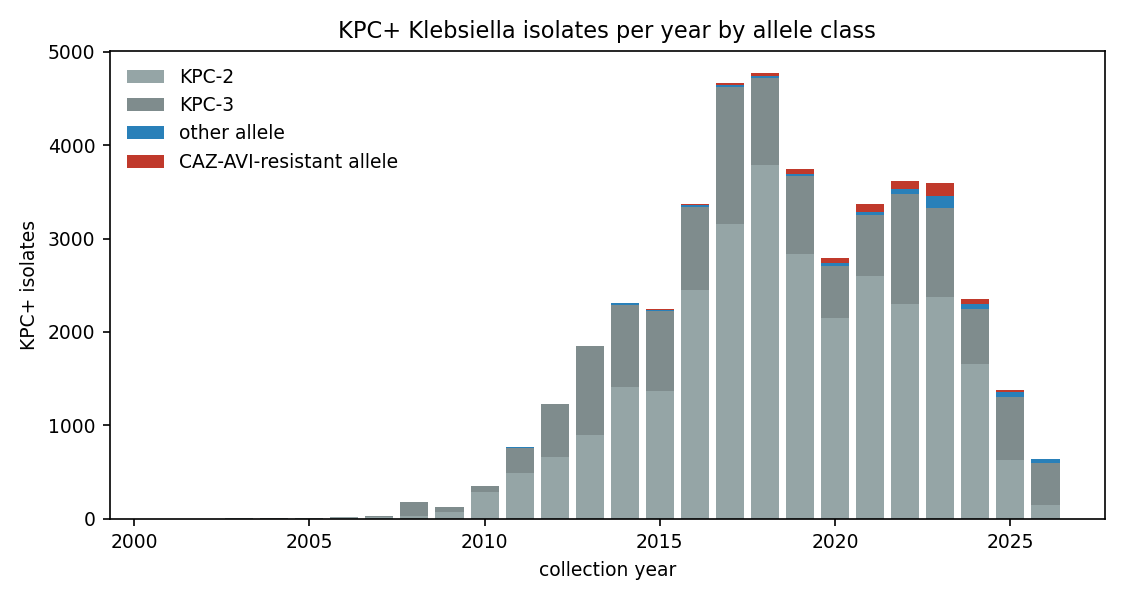
\includegraphics[width=0.95\textwidth]{../results/figures/F2_yearly_class.png}\caption{KPC$^+$ isolates per collection year by allele class. Documented CAZ-AVI-resistant alleles (red) rise from 0\% (pre-2013) to 3.8\% (2023); recent years underreported.}\end{figure}
\begin{figure}[t]\centering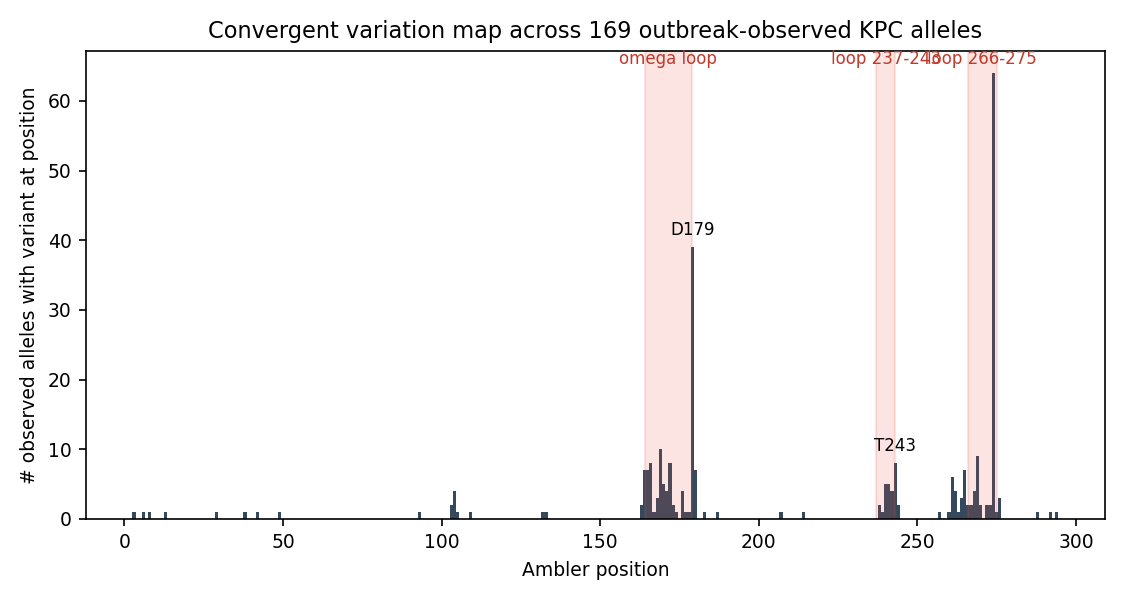
\includegraphics[width=0.95\textwidth]{../results/figures/F3_variation_map.png}\caption{Convergence map: number of circulating alleles carrying a variant at each Ambler position. Red bands: the three resistance hot spots.}\end{figure}
\begin{figure}[t]\centering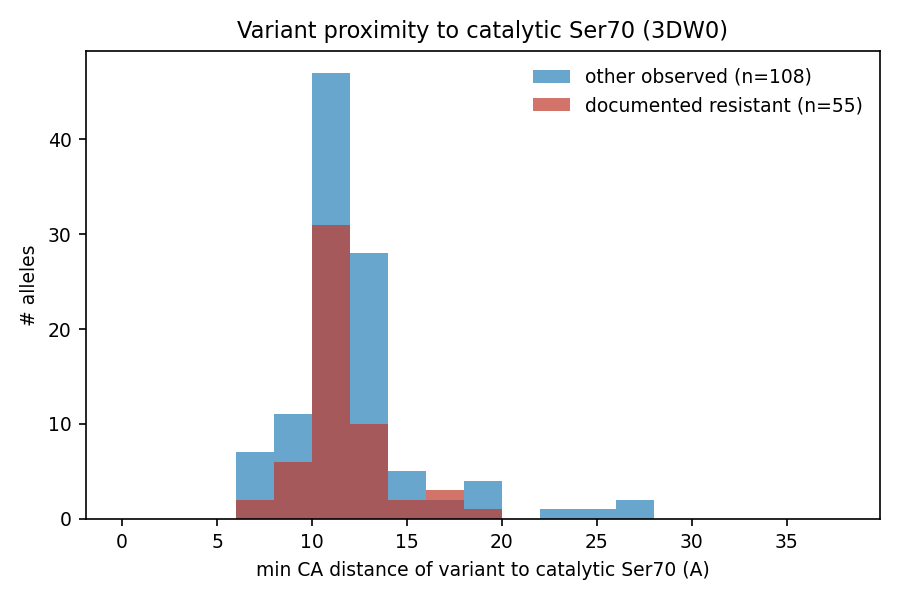
\includegraphics[width=0.6\textwidth]{../results/figures/F4_dist_s70.png}\caption{Minimum variant-to-Ser70 C$\alpha$ distance does not separate documented-resistant from other circulating alleles ($p=0.122$).}\end{figure}
\begin{figure}[t]\centering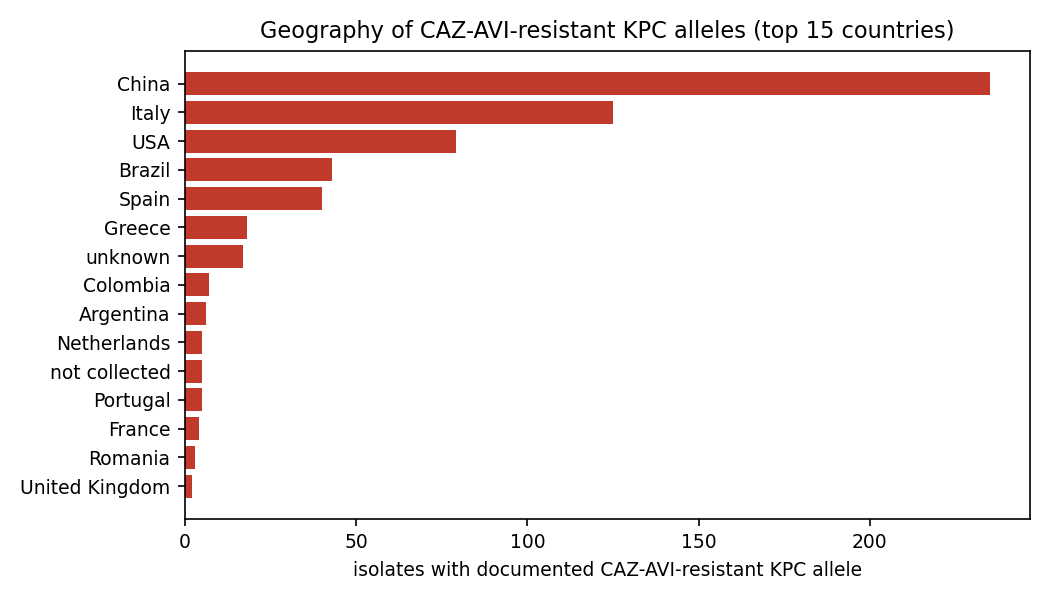
\includegraphics[width=0.7\textwidth]{../results/figures/F5_geo_resistant.png}\caption{Countries contributing the most isolates with documented CAZ-AVI-resistant KPC alleles.}\end{figure}

\clearpage
\section{Discussion}
Three conclusions follow. First, KPC's escape from CAZ-AVI is not idiosyncratic: at outbreak scale it reuses a small set of structural routes, all remodeling one of three pocket-lining loops. That convergence is good news for surveillance and for inhibitor design - the escape space is bounded and enumerable, and 39-allele convergence at D179 marks the single most important watch position.

Second, validated calling matters. Our caller passed a locked 100\% exact-reproduction gate on 526 allele records spanning two databases before touching outbreak data, and the two reference databases proved perfectly consistent on their 230 shared alleles. That makes the downstream atlas a measurement, not an estimate. The same discipline surfaced a real operational finding: 18 circulating alleles postdate the CARD snapshot, nine with loop insertions at documented resistance positions.

Third, structure helps where naive geometry fails. The distance-to-Ser70 negative result shows that simple proximity scores would misfire on KPC, while loop-level features (membership, indel type) and the B-factor destabilization signature reproduce the mechanism. A practical next step is a per-allele risk score combining loop membership, indel length, and loop-order proxies, calibrated on the 65-variant documented set.

\textit{Limitations.} The census inherits Pathogen Detection sampling biases (country and year coverage, submission lag depressing 2024--2026). Allele calls are AMRFinderPlus-derived; the 649 unnamed/partial calls were not re-extracted from assemblies, so rare novel proteins may hide there. Resistance grading relies on a literature-curated set; alleles graded ``hypothesis'' require phenotypic confirmation, and MIC data are not part of the snapshot. Structural annotation uses WT and D179-background structures; allele-specific conformations (especially large indels) are approximations.

\section{Data and code availability}
Code, manifests with SHA-256 byte-locks, the 296-allele union reference set, the master allele table and all figures: repository \texttt{amr-carbapenem-structure}, directory \texttt{kpc/}. All sources are public (NCBI Pathogen Detection, AMRFinderPlus, CARD, RCSB PDB, PMC).

\begin{thebibliography}{19}\small
\bibitem{pd} NCBI Pathogen Detection Isolates Browser, Klebsiella group snapshot PDG000000012.2532. \texttt{https://www.ncbi.nlm.nih.gov/pathogens/}
\bibitem{amrfinder} Feldgarden M, et al. AMRFinderPlus and the Reference Gene Catalog. \emph{Sci Rep} 2021;11:12728.
\bibitem{card} Alcock BP, et al. CARD 2023. \emph{Nucleic Acids Res} 2023;51:D690--D699.
\bibitem{review1} Gona F, et al. Klebsiella pneumoniae carbapenemase variants resistant to ceftazidime-avibactam: an evolutionary overview. \emph{Antibiotics} 2022 (PMC9487638).
\bibitem{review2} The Klebsiella pneumoniae carbapenemase (KPC) $\beta$-lactamase has evolved in response to ceftazidime-avibactam. \emph{mBio} 2024 (PMC10812414).
\bibitem{d179struct} Tooke CL, et al. Structural characterization of the D179N and D179Y variants of KPC-2: omega-loop destabilization as a mechanism of resistance to ceftazidime-avibactam. \emph{Antimicrob Agents Chemother} 2021;65:e02414-21.
\bibitem{d179eng} Papp-Wallace KM, et al. KPC-2, substitutions at Ambler position Asp179, and resistance to ceftazidime-avibactam. \emph{mBio} 2017;8:e00528-17.
\bibitem{indel} KPC beta-lactamases are permissive to insertions and deletions conferring substrate spectrum modifications and resistance to ceftazidime-avibactam. \emph{Antimicrob Agents Chemother} 2020 (aac.01175-20).
\bibitem{hotspot261} Repeated insertions at positions 261--280 in KPC-2 highlight a ceftazidime-avibactam resistance hotspot (KPC-261). \emph{iScience} 2026 (10.1016/j.isci.2026.116514).
\bibitem{surv} A large-scale surveillance revealed that KPC variants mediated ceftazidime-avibactam resistance in clinically isolated Klebsiella pneumoniae. \emph{Microbiol Spectr} 2024 (spectrum.00258-24).
\bibitem{4zbe} Krishnan NP, et al. Inhibition of Klebsiella $\beta$-lactamases (SHV-1 and KPC-2) by avibactam: a structural study. \emph{PLoS One} 2015;10:e0136813 (PDB 4ZBE).
\bibitem{3dw0} PDB 3DW0: crystal structure of the class A carbapenemase KPC-2 at 1.6 \AA. RCSB Protein Data Bank.
\bibitem{acyl} PDB 8AKK/8AKL: acyl-enzyme complexes of imipenem and meropenem with KPC-2 E166Q. RCSB Protein Data Bank.
\bibitem{kpc204} Identification of a novel KPC variant, KPC-204, conferring resistance to both carbapenems and ceftazidime-avibactam in ST11 K. pneumoniae. \emph{Microorganisms} 2024;12:1193.
\bibitem{l169p} Ceftazidime/avibactam resistance associated with L169P mutation in the omega loop of KPC-2. \emph{J Antimicrob Chemother} (reviewed in ref 5).
\end{thebibliography}

\clearpage
\footnotesize\begin{longtable}{@{}l p{5.2cm} r p{2.6cm} l l@{}}
\caption{Outbreak-observed KPC alleles with documented ceftazidime-avibactam resistance (55 of 65 documented alleles observed). Ambler numbering anchored to PDB 3DW0.}\\
\hline Allele & Variant signature (Ambler) & Isolates & Hotspot & Top country & Years \\\hline\endhead
\hline\multicolumn{6}{r}{continued}\\\endfoot
\hline\endlastfoot
KPC-33 & D179Y & 173 & omega\_loop & China & 2016-2025 \\
KPC-31 & D179Y; H274Y & 118 & loop266\_275;omega\_loop & Italy & 2014-2026 \\
KPC-71 & ins180\_S & 42 & - & China & 2017-2025 \\
KPC-23 & V240A; H274Y & 36 & loop237\_243;loop266\_275 & Greece & 2014-2025 \\
KPC-66 & del166\_EL; H274Y & 22 & loop266\_275;omega\_loop & Italy & 2019-2024 \\
KPC-8 & V240G; H274Y & 20 & loop237\_243;loop266\_275 & USA & 2013-2021 \\
KPC-14 & del242\_GT & 16 & loop237\_243 & China & 2003-2024 \\
KPC-25 & ins165\_EL & 12 & omega\_loop & China & 2020-2025 \\
KPC-62 & L169Q; H274Y & 11 & loop266\_275;omega\_loop & Spain & 2019-2023 \\
KPC-72 & A172D & 10 & omega\_loop & China & 2017-2023 \\
KPC-84 & T243P & 10 & loop237\_243 & China & 2016-2025 \\
KPC-68 & ins180\_SS; H274Y & 9 & loop266\_275 & USA & 2019-2026 \\
KPC-44 & ins261\_AVYTRAPNKDDKHSE & 8 & - & China & 2020-2024 \\
KPC-90 & ins179\_TY & 8 & omega\_loop & China & 2018-2025 \\
KPC-46 & L169P; H274Y & 7 & loop266\_275;omega\_loop & Portugal & 2019-2024 \\
KPC-49 & R164S; H274Y & 7 & loop266\_275;omega\_loop & Italy & 2018-2024 \\
KPC-53 & ins165\_EL; H274Y & 7 & loop266\_275;omega\_loop & Italy & 2016-2026 \\
KPC-29 & ins269\_KDD; H274Y & 6 & loop266\_275 & USA & 2019-2024 \\
KPC-35 & L169P & 6 & omega\_loop & China & 2020-2022 \\
KPC-78 & D179A & 6 & omega\_loop & China & 2019-2023 \\
KPC-39 & A172T; H274Y & 5 & loop266\_275;omega\_loop & France & 2018-2024 \\
KPC-88 & D176Y & 5 & omega\_loop & China & 2017-2023 \\
KPC-65 & ins179\_TY; H274Y & 4 & loop266\_275;omega\_loop & USA & 2017-2023 \\
KPC-86 & D179G & 4 & omega\_loop & China & 2022-2023 \\
KPC-50 & H274Y; ins275\_EAV & 3 & loop266\_275 & USA & 2024-2025 \\
KPC-57 & D179V & 3 & omega\_loop & China & 2020-2022 \\
KPC-67 & ins269\_KDDKDD; H274Y & 3 & loop266\_275 & Italy & 2019-2020 \\
KPC-76 & D179Y; ins262\_VYTRAPN & 3 & omega\_loop & China & 2019-2022 \\
KPC-85 & A172V; H274Y & 3 & loop266\_275;omega\_loop & Netherlands & 2018-2021 \\
KPC-94 & del169\_L; N170H; H274Y & 3 & loop266\_275;omega\_loop & Italy & 2017-2024 \\
KPC-32 & D179Y; T243M; H274Y & 2 & loop237\_243;loop266\_275;omega\_loop & USA & 2015-2015 \\
KPC-36 & D163E; H274Y & 2 & loop266\_275 & Italy & 2017-2019 \\
KPC-41 & ins267\_PNK; H274Y & 2 & loop266\_275 & not collected & 2018-2018 \\
KPC-74 & del239\_GV & 2 & loop237\_243 & China & 2020-2025 \\
KPC-79 & ins262\_VYTRAPN & 2 & - & China & 2019-2022 \\
KPC-103 & ins269\_KDDKHSEAVIAA & 2 & loop266\_275 & Brazil & 2019-2019 \\
KPC-112 & del166\_EL; del242\_GT & 2 & loop237\_243;omega\_loop & China & 2023-2024 \\
KPC-114 & ins180\_SS & 2 & - & unknown & 2020-2023 \\
KPC-51 & D179N; Y241H; H274N & 1 & loop237\_243;loop266\_275;omega\_loop & China & 2018-2018 \\
KPC-52 & D179Y; ins262\_V & 1 & omega\_loop & China & 2018-2018 \\
KPC-58 & ins265\_RAPNKDDN & 1 & - & Croatia & 2019-2019 \\
KPC-69 & ins165\_GL; H274Y & 1 & loop266\_275;omega\_loop & Italy & 2020-2020 \\
KPC-70 & D179Y; T265A; H274Y & 1 & loop266\_275;omega\_loop & Italy & 2020-2020 \\
KPC-80 & ins267\_PNK & 1 & loop266\_275 & Argentina & 2019-2019 \\
KPC-95 & A172T; D179Y; H274Y & 1 & loop266\_275;omega\_loop & Spain & 2018-2018 \\
KPC-96 & Y241N & 1 & loop237\_243 & Argentina & 2019-2019 \\
KPC-97 & ins274\_SEAVN & 1 & loop266\_275 & Argentina & 2020-2020 \\
KPC-98 & R164H; H274Y & 1 & loop266\_275;omega\_loop & Italy & 2023-2023 \\
KPC-104 & ins179\_TY; ins270\_DDKHSE & 1 & loop266\_275;omega\_loop & Brazil & 2020-2020 \\
KPC-105 & L169Q; ins261\_AVYTRAPNKDDKHSE & 1 & omega\_loop & Brazil & 2020-2020 \\
KPC-106 & ins179\_TY; ins274\_SEAV & 1 & loop266\_275;omega\_loop & Brazil & 2021-2021 \\
KPC-107 & ins180\_SSPRAVTESLQKLTLGSALAAPQRQQFV & 1 & - & Brazil & 2020-2020 \\
KPC-108 & ins179\_TSSPRAVTEN; ins261\_AVYTRAPNKDDKHSE & 1 & omega\_loop & Brazil & 2021-2021 \\
KPC-113 & ins266\_G & 1 & loop266\_275 & Brazil & 2020-2020 \\
KPC-115 & del169\_LN; S171P; H274Y & 1 & loop266\_275;omega\_loop & Argentina & 2021-2021 \\
\end{longtable}

\clearpage
\footnotesize\begin{longtable}{@{}l p{5.6cm} r l l@{}}
\caption{Outbreak-observed alleles present in AMRFinderPlus 2026-08-07.1 but absent from the CARD 2026-09-23 snapshot (post-CARD named alleles).}\\
\hline Allele & Variant signature (Ambler) & Isolates & Top country & Years \\\hline\endhead
\hline\multicolumn{5}{r}{continued}\\\endfoot
\hline\endlastfoot
KPC-244 & N214T & 3 & USA & 2016-2019 \\
KPC-250 & D179Y; ins268\_N & 2 & China & 2023-2023 \\
KPC-262 & P268S & 2 & China & 2022-2024 \\
KPC-264 & S109P & 2 & China & 2016-2025 \\
KPC-275 & D179Y; T243P & 2 & China & 2025-2025 \\
KPC-276 & T243A; H274Y & 2 & USA & 2015-2018 \\
KPC-245 & ins263\_YTRAPNKDD; H274Y; E276D & 1 & Italy & 2024-2024 \\
KPC-252 & ins243\_ANDYAA & 1 & China & 2022-2022 \\
KPC-259 & ins264\_TRAPN & 1 & USA & 2017-2017 \\
KPC-261 & D179Y; ins266\_APNKDE & 1 & China & 2021-2021 \\
KPC-263 & ins238\_G & 1 & China & 2018-2018 \\
KPC-272 & ins165\_EL; ins273\_YSEAV; H274N & 1 & unknown & 2025-2025 \\
KPC-281 & A257S & 1 & Slovakia & 2025-2025 \\
KPC-282 & ins264\_TRAPNK & 1 & Italy & 2023-2023 \\
KPC-287 & L169Q; del242\_GT & 1 & China & 2025-2025 \\
KPC-295 & ins165\_EL; T243A; H274Y & 1 & Italy & 2022-2022 \\
KPC-297 & ins168\_LK; del242\_GT & 1 & China & 2025-2025 \\
KPC-300 & P268T; H274R & 1 & China & 2022-2022 \\
\end{longtable}


\clearpage
\appendix
\section{Full outbreak census of 169 observed KPC alleles}
\footnotesize\begin{longtable}{@{}l p{4.6cm} r r l l l@{}}
\caption{Complete census of the 169 outbreak-observed KPC alleles (snapshot PDG000000012.2532). Distance = minimum C$\alpha$ distance of any variant to Ser70 (3DW0).}\\
\hline Allele & Signature (Ambler) & Isolates & Dist (\AA) & Grade & Top country & Years \\\hline\endhead
\hline\multicolumn{7}{r}{continued}\\\endfoot
\hline\endlastfoot
KPC-2 & identical to KPC-2 & 34616 & - & no evidence & China & 1996-2026 \\
KPC-3 & H274Y & 13788 & 13.9 & hypothesis & USA & 2001-2026 \\
KPC-33 & D179Y & 173 & 10.0 & documented & China & 2016-2025 \\
KPC-31 & D179Y; H274Y & 118 & 10.0 & documented & Italy & 2014-2026 \\
KPC-4 & P104R; V240G & 108 & 12.9 & hypothesis & USA & 2011-2026 \\
KPC-144 & A172T & 52 & 11.5 & hypothesis & China & 2018-2023 \\
KPC-6 & V240G & 51 & 12.9 & hypothesis & USA & 2014-2026 \\
KPC-71 & ins180\_S & 42 & 10.9 & documented & China & 2017-2025 \\
KPC-12 & L169M & 36 & 8.8 & hypothesis & China & 2014-2024 \\
KPC-23 & V240A; H274Y & 36 & 12.9 & documented & Greece & 2014-2025 \\
KPC-18 & V8I & 30 & - & no evidence & USA & 2016-2026 \\
KPC-66 & del166\_EL; H274Y & 22 & 8.9 & documented & Italy & 2019-2024 \\
KPC-8 & V240G; H274Y & 20 & 12.9 & documented & USA & 2013-2021 \\
KPC-181 & E276D & 19 & 14.7 & no evidence & Brazil & 2016-2025 \\
KPC-14 & del242\_GT & 16 & 10.9 & documented & China & 2003-2024 \\
KPC-17 & F207L & 16 & 16.2 & no evidence & Taiwan & 2014-2024 \\
KPC-5 & P104R & 14 & 13.1 & no evidence & USA & 2014-2026 \\
KPC-157 & N132S & 13 & 8.4 & hypothesis & China & 2016-2024 \\
KPC-25 & ins165\_EL & 12 & 10.6 & documented & China & 2020-2025 \\
KPC-62 & L169Q; H274Y & 11 & 8.8 & documented & Spain & 2019-2023 \\
KPC-72 & A172D & 10 & 11.5 & documented & China & 2017-2023 \\
KPC-84 & T243P & 10 & 10.9 & documented & China & 2016-2025 \\
KPC-56 & H274Y; G294W & 9 & 13.9 & hypothesis & USA & 2013-2022 \\
KPC-68 & ins180\_SS; H274Y & 9 & 10.9 & documented & USA & 2019-2026 \\
KPC-166 & del169\_L; N170H & 9 & 7.9 & hypothesis & Italy & 2014-2022 \\
KPC-170 & D179N & 9 & 10.0 & hypothesis & China & 2017-2023 \\
KPC-173 & ins168\_LK & 9 & 11.4 & hypothesis & China & 2016-2023 \\
KPC-44 & ins261\_AVYTRAPNKDDKHSE & 8 & 16.6 & documented & China & 2020-2024 \\
KPC-90 & ins179\_TY & 8 & 10.0 & documented & China & 2018-2025 \\
KPC-93 & ins265\_RAPNN & 8 & 13.2 & no evidence & China & 2021-2023 \\
KPC-184 & H274Y; E276D & 8 & 13.9 & hypothesis & Italy & 2019-2026 \\
KPC-10 & P104R; H274Y & 7 & 13.1 & hypothesis & USA & 2014-2025 \\
KPC-46 & L169P; H274Y & 7 & 8.8 & documented & Portugal & 2019-2024 \\
KPC-49 & R164S; H274Y & 7 & 11.9 & documented & Italy & 2018-2024 \\
KPC-53 & ins165\_EL; H274Y & 7 & 10.6 & documented & Italy & 2016-2026 \\
KPC-148 & ins261\_AVYTRAPNKDDKYSE; H274Y & 7 & 13.9 & hypothesis & USA & 2015-2024 \\
KPC-176 & S171P & 7 & 11.6 & hypothesis & China & 2017-2024 \\
KPC-29 & ins269\_KDD; H274Y & 6 & 13.9 & documented & USA & 2019-2024 \\
KPC-35 & L169P & 6 & 8.8 & documented & China & 2020-2022 \\
KPC-78 & D179A & 6 & 10.0 & documented & China & 2019-2023 \\
KPC-204 & ins269\_KDD & 6 & 19.9 & hypothesis & China & 2017-2023 \\
KPC-227 & D179Y; ins269\_KDD & 6 & 10.0 & hypothesis & China & 2023-2023 \\
KPC-39 & A172T; H274Y & 5 & 11.5 & documented & France & 2018-2024 \\
KPC-88 & D176Y & 5 & 16.6 & documented & China & 2017-2023 \\
KPC-130 & D179G; H274Y & 5 & 10.0 & hypothesis & Italy & 2020-2026 \\
KPC-160 & del166\_EL & 5 & 8.9 & hypothesis & China & 2021-2024 \\
KPC-212 & R164L & 5 & 11.9 & hypothesis & China & 2023-2023 \\
KPC-27 & W105R; H274Y & 4 & 11.0 & hypothesis & Spain & 2013-2014 \\
KPC-65 & ins179\_TY; H274Y & 4 & 10.0 & documented & USA & 2017-2023 \\
KPC-86 & D179G & 4 & 10.0 & documented & China & 2022-2023 \\
KPC-126 & A172V & 4 & 11.5 & hypothesis & China & 2020-2023 \\
KPC-145 & D179Y; T265A & 4 & 10.0 & hypothesis & China & 2023-2024 \\
KPC-167 & D179Y; ins270\_DDKYSE; H274Y & 4 & 10.0 & hypothesis & Italy & 2021-2022 \\
KPC-168 & D176N & 4 & 16.6 & hypothesis & China & 2016-2023 \\
KPC-38 & H274Y; V292A & 3 & 13.9 & hypothesis & USA & 2015-2025 \\
KPC-50 & H274Y; ins275\_EAV & 3 & 13.9 & documented & USA & 2024-2025 \\
KPC-57 & D179V & 3 & 10.0 & documented & China & 2020-2022 \\
KPC-61 & S171P; H274Y & 3 & 11.6 & hypothesis & Brazil & 2020-2020 \\
KPC-67 & ins269\_KDDKDD; H274Y & 3 & 13.9 & documented & Italy & 2019-2020 \\
KPC-76 & D179Y; ins262\_VYTRAPN & 3 & 10.0 & documented & China & 2019-2022 \\
KPC-85 & A172V; H274Y & 3 & 11.5 & documented & Netherlands & 2018-2021 \\
KPC-92 & del166\_EL; N170D; H274Y & 3 & 7.9 & hypothesis & Spain & 2020-2020 \\
KPC-94 & del169\_L; N170H; H274Y & 3 & 7.9 & documented & Italy & 2017-2024 \\
KPC-100 & T243M & 3 & 10.9 & hypothesis & China & 2022-2023 \\
KPC-121 & ins180\_S; H274Y & 3 & 10.9 & hypothesis & Italy & 2021-2023 \\
KPC-154 & ins265\_RAPNKDDKYS; H274Y & 3 & 13.2 & hypothesis & Italy & 2022-2022 \\
KPC-172 & D179E & 3 & 10.0 & hypothesis & China & 2016-2017 \\
KPC-205 & ins265\_RAPNN; H274Y & 3 & 13.2 & hypothesis & Italy & 2022-2025 \\
KPC-239 & del240\_V; Y241D; H274Y & 3 & 12.9 & hypothesis & Italy & 2022-2023 \\
KPC-244 & N214T & 3 & 12.6 & no evidence & USA & 2016-2019 \\
KPC-30 & R6H & 2 & - & no evidence & Brazil & 2016-2016 \\
KPC-32 & D179Y; T243M; H274Y & 2 & 10.0 & documented & USA & 2015-2015 \\
KPC-36 & D163E; H274Y & 2 & 13.2 & documented & Italy & 2017-2019 \\
KPC-41 & ins267\_PNK; H274Y & 2 & 13.9 & documented & not collected & 2018-2018 \\
KPC-74 & del239\_GV & 2 & 10.6 & documented & China & 2020-2025 \\
KPC-75 & L13F & 2 & - & no evidence & China & 2019-2019 \\
KPC-79 & ins262\_VYTRAPN & 2 & 13.6 & documented & China & 2019-2022 \\
KPC-81 & del173\_I & 2 & 15.3 & hypothesis & Argentina & 2020-2020 \\
KPC-99 & R164S & 2 & 11.9 & hypothesis & Romania & 2020-2023 \\
KPC-103 & ins269\_KDDKHSEAVIAA & 2 & 19.9 & documented & Brazil & 2019-2019 \\
KPC-112 & del166\_EL; del242\_GT & 2 & 8.9 & documented & China & 2023-2024 \\
KPC-114 & ins180\_SS & 2 & 10.9 & documented & unknown & 2020-2023 \\
KPC-118 & V103L; W165R; H274Y & 2 & 10.6 & hypothesis & USA & 2020-2021 \\
KPC-124 & del166\_EL; D179Y; H274Y & 2 & 8.9 & hypothesis & Portugal & 2022-2022 \\
KPC-125 & D179A; H274Y & 2 & 10.0 & hypothesis & Italy & 2021-2025 \\
KPC-127 & ins165\_EL; A172T & 2 & 10.6 & hypothesis & China & 2022-2025 \\
KPC-141 & D179Y; ins238\_G & 2 & 7.3 & hypothesis & Brazil & 2021-2022 \\
KPC-179 & A133T; ins180\_S & 2 & 10.9 & no evidence & China & 2023-2023 \\
KPC-180 & R164H & 2 & 11.9 & hypothesis & China & 2022-2023 \\
KPC-190 & D179Y; A244V & 2 & 8.9 & hypothesis & China & 2024-2024 \\
KPC-203 & del166\_EL; ins260\_LAVYTRAPM; H274Y & 2 & 8.9 & hypothesis & Italy & 2022-2022 \\
KPC-216 & ins169\_K; H274Y & 2 & 8.8 & hypothesis & Italy & 2022-2022 \\
KPC-250 & D179Y; ins268\_N & 2 & 10.0 & hypothesis & China & 2023-2023 \\
KPC-262 & P268S & 2 & 19.7 & hypothesis & China & 2022-2024 \\
KPC-264 & S109P & 2 & 15.7 & no evidence & China & 2016-2025 \\
KPC-275 & D179Y; T243P & 2 & 10.0 & hypothesis & China & 2025-2025 \\
KPC-276 & T243A; H274Y & 2 & 10.9 & hypothesis & USA & 2015-2018 \\
KPC-7 & M49I; H274Y & 1 & 13.9 & hypothesis & unknown & - \\
KPC-11 & P104L & 1 & 13.1 & no evidence & unknown & - \\
KPC-20 & V29I & 1 & - & no evidence & USA & 2017-2017 \\
KPC-45 & T93K & 1 & 23.6 & no evidence & USA & 2020-2020 \\
KPC-51 & D179N; Y241H; H274N & 1 & 10.0 & documented & China & 2018-2018 \\
KPC-52 & D179Y; ins262\_V & 1 & 10.0 & documented & China & 2018-2018 \\
KPC-58 & ins265\_RAPNKDDN & 1 & 13.2 & documented & Croatia & 2019-2019 \\
KPC-69 & ins165\_GL; H274Y & 1 & 10.6 & documented & Italy & 2020-2020 \\
KPC-70 & D179Y; T265A; H274Y & 1 & 10.0 & documented & Italy & 2020-2020 \\
KPC-77 & R164P & 1 & 11.9 & hypothesis & China & 2022-2022 \\
KPC-80 & ins267\_PNK & 1 & 17.2 & documented & Argentina & 2019-2019 \\
KPC-91 & V103L; H274Y & 1 & 13.9 & hypothesis & Taiwan & 2020-2020 \\
KPC-95 & A172T; D179Y; H274Y & 1 & 10.0 & documented & Spain & 2018-2018 \\
KPC-96 & Y241N & 1 & 14.6 & documented & Argentina & 2019-2019 \\
KPC-97 & ins274\_SEAVN & 1 & 13.9 & documented & Argentina & 2020-2020 \\
KPC-98 & R164H; H274Y & 1 & 11.9 & documented & Italy & 2023-2023 \\
KPC-101 & ins272\_KH & 1 & 18.2 & hypothesis & China & 2023-2023 \\
KPC-104 & ins179\_TY; ins270\_DDKHSE & 1 & 10.0 & documented & Brazil & 2020-2020 \\
KPC-105 & L169Q; ins261\_AVYTRAPNKDDKHSE & 1 & 8.8 & documented & Brazil & 2020-2020 \\
KPC-106 & ins179\_TY; ins274\_SEAV & 1 & 10.0 & documented & Brazil & 2021-2021 \\
KPC-107 & ins180\_SSPRAVTESLQKLTLGSALAAPQRQQFV & 1 & 10.9 & documented & Brazil & 2020-2020 \\
KPC-108 & ins179\_TSSPRAVTEN; ins261\_AVYTRAPNKDDKHSE & 1 & 10.0 & documented & Brazil & 2021-2021 \\
KPC-109 & ins268\_NKDDKY; H274Y & 1 & 13.9 & hypothesis & Italy & 2021-2021 \\
KPC-110 & G42R; D179Y; H274Y & 1 & 10.0 & hypothesis & Italy & 2021-2021 \\
KPC-113 & ins266\_G & 1 & 14.1 & documented & Brazil & 2020-2020 \\
KPC-115 & del169\_LN; S171P; H274Y & 1 & 7.9 & documented & Argentina & 2021-2021 \\
KPC-119 & Q38H & 1 & 25.3 & no evidence & USA & 2018-2018 \\
KPC-128 & D179Y; T243M & 1 & 10.0 & hypothesis & China & 2022-2022 \\
KPC-129 & N170H; ins262\_VYTRAPNK & 1 & 7.9 & hypothesis & China & 2022-2022 \\
KPC-132 & ins265\_RAPNKDDKS; H274Y & 1 & 13.2 & hypothesis & Spain & 2022-2022 \\
KPC-135 & del166\_EL; ins261\_AVYTRAPNKDDKHSE & 1 & 8.9 & hypothesis & China & 2023-2023 \\
KPC-139 & D179Y; ins269\_KDDKHS & 1 & 10.0 & hypothesis & Brazil & 2020-2020 \\
KPC-140 & D179N; ins261\_AVYTRAPNKDDKHSE & 1 & 10.0 & hypothesis & Brazil & 2021-2021 \\
KPC-142 & ins180\_S; ins272\_KHSEAV & 1 & 10.9 & hypothesis & Brazil & 2021-2021 \\
KPC-143 & D179Y; T187S & 1 & 10.0 & hypothesis & Brazil & 2021-2021 \\
KPC-146 & L3M & 1 & - & no evidence & China & - \\
KPC-150 & del167\_LEL; N170H; H274Y & 1 & 7.9 & hypothesis & Spain & - \\
KPC-158 & A244V & 1 & 8.9 & hypothesis & China & 2017-2017 \\
KPC-162 & ins264\_TRAPNKD & 1 & 11.9 & no evidence & Argentina & 2022-2022 \\
KPC-163 & ins269\_KDDKHS & 1 & 19.9 & hypothesis & Argentina & 2022-2022 \\
KPC-169 & del176\_DAR & 1 & 13.6 & hypothesis & China & 2017-2017 \\
KPC-171 & ins274\_SEAVIAAD & 1 & 13.9 & hypothesis & China & 2017-2017 \\
KPC-174 & del241\_Y & 1 & 14.6 & hypothesis & China & 2019-2019 \\
KPC-175 & ins179\_T & 1 & 10.0 & hypothesis & China & 2019-2019 \\
KPC-177 & ins179\_TSSPRAVTESLQN & 1 & 10.0 & hypothesis & China & 2016-2016 \\
KPC-178 & P174L; H274Y & 1 & 13.9 & hypothesis & USA & 2018-2018 \\
KPC-183 & ins269\_KDDKYS; H274Y & 1 & 13.9 & hypothesis & Italy & 2019-2019 \\
KPC-189 & A172T; D179Y & 1 & 10.0 & hypothesis & China & 2023-2023 \\
KPC-194 & D179Y; P183L & 1 & 10.0 & hypothesis & China & 2023-2023 \\
KPC-195 & E288D & 1 & 26.8 & no evidence & USA & 2011-2011 \\
KPC-197 & del166\_EL; A177E; ins273\_YS; H274D & 1 & 8.9 & hypothesis & Colombia & 2023-2023 \\
KPC-202 & ins274\_SEAVIAAAAN & 1 & 13.9 & hypothesis & China & 2023-2023 \\
KPC-211 & del176\_DARD & 1 & 10.0 & hypothesis & China & 2023-2023 \\
KPC-213 & D163G & 1 & 13.2 & no evidence & China & 2023-2023 \\
KPC-214 & R178H & 1 & 13.6 & hypothesis & China & 2023-2023 \\
KPC-215 & I173S & 1 & 15.3 & hypothesis & China & 2023-2023 \\
KPC-228 & del168\_ELNS & 1 & 7.9 & hypothesis & China & 2021-2021 \\
KPC-230 & R164S; ins269\_KDDKHS & 1 & 11.9 & hypothesis & China & 2024-2024 \\
KPC-231 & S171Y; H274Y & 1 & 11.6 & hypothesis & Italy & 2022-2022 \\
KPC-234 & D179G; Y241D & 1 & 10.0 & hypothesis & China & 2023-2023 \\
KPC-245 & ins263\_YTRAPNKDD; H274Y; E276D & 1 & 13.5 & hypothesis & Italy & 2024-2024 \\
KPC-252 & ins243\_ANDYAA & 1 & 10.9 & hypothesis & China & 2022-2022 \\
KPC-259 & ins264\_TRAPN & 1 & 11.9 & no evidence & USA & 2017-2017 \\
KPC-261 & D179Y; ins266\_APNKDE & 1 & 10.0 & hypothesis & China & 2021-2021 \\
KPC-263 & ins238\_G & 1 & 7.3 & hypothesis & China & 2018-2018 \\
KPC-272 & ins165\_EL; ins273\_YSEAV; H274N & 1 & 10.6 & hypothesis & unknown & 2025-2025 \\
KPC-281 & A257S & 1 & 27.5 & no evidence & Slovakia & 2025-2025 \\
KPC-282 & ins264\_TRAPNK & 1 & 11.9 & no evidence & Italy & 2023-2023 \\
KPC-287 & L169Q; del242\_GT & 1 & 8.8 & hypothesis & China & 2025-2025 \\
KPC-295 & ins165\_EL; T243A; H274Y & 1 & 10.6 & hypothesis & Italy & 2022-2022 \\
KPC-297 & ins168\_LK; del242\_GT & 1 & 10.9 & hypothesis & China & 2025-2025 \\
KPC-300 & P268T; H274R & 1 & 13.9 & hypothesis & China & 2022-2022 \\
\end{longtable}

\clearpage
\section{Convergent Ambler positions across circulating alleles}
\small\begin{longtable}{llp{9cm}}
\caption{Convergent Ambler positions: all positions varied in at least two independent circulating alleles.}\\
\hline Ambler position & \# alleles & Alleles \\\hline\endhead
\hline \multicolumn{3}{r}{continued}\\\endfoot
\hline\endlastfoot
274 & 64 & KPC-3, KPC-7, KPC-8, KPC-10, KPC-23, KPC-27, KPC-29, KPC-31, KPC-32, KPC-36, KPC-38, KPC-39, KPC-41, KPC-46, KPC-49, KPC-50, KPC-51, KPC-53, KPC-56, KPC-61, KPC-62, KPC-65, KPC-66, KPC-67, KPC-68, KPC-69, KPC-70, KPC-85, KPC-91, KPC-92, KPC-94, KPC-95, KPC-97, KPC-98, KPC-106, KPC-109, KPC-110, KPC-115, KPC-118, KPC-121, KPC-124, KPC-125, KPC-130, KPC-132, KPC-148, KPC-150, KPC-154, KPC-167, KPC-171, KPC-178, KPC-183, KPC-184, KPC-197, KPC-202, KPC-203, KPC-205, KPC-216, KPC-231, KPC-239, KPC-245, KPC-272, KPC-276, KPC-295, KPC-300 \\
179 & 39 & KPC-31, KPC-32, KPC-33, KPC-51, KPC-52, KPC-57, KPC-65, KPC-70, KPC-76, KPC-78, KPC-86, KPC-90, KPC-95, KPC-104, KPC-106, KPC-108, KPC-110, KPC-124, KPC-125, KPC-128, KPC-130, KPC-139, KPC-140, KPC-141, KPC-143, KPC-145, KPC-167, KPC-170, KPC-172, KPC-175, KPC-177, KPC-189, KPC-190, KPC-194, KPC-227, KPC-234, KPC-250, KPC-261, KPC-275 \\
169 & 10 & KPC-12, KPC-35, KPC-46, KPC-62, KPC-94, KPC-105, KPC-115, KPC-166, KPC-216, KPC-287 \\
269 & 9 & KPC-29, KPC-67, KPC-103, KPC-139, KPC-163, KPC-183, KPC-204, KPC-227, KPC-230 \\
172 & 8 & KPC-39, KPC-72, KPC-85, KPC-95, KPC-126, KPC-127, KPC-144, KPC-189 \\
166 & 8 & KPC-66, KPC-92, KPC-112, KPC-124, KPC-135, KPC-160, KPC-197, KPC-203 \\
243 & 8 & KPC-32, KPC-84, KPC-100, KPC-128, KPC-252, KPC-275, KPC-276, KPC-295 \\
180 & 7 & KPC-68, KPC-71, KPC-107, KPC-114, KPC-121, KPC-142, KPC-179 \\
165 & 7 & KPC-25, KPC-53, KPC-69, KPC-118, KPC-127, KPC-272, KPC-295 \\
265 & 7 & KPC-58, KPC-70, KPC-93, KPC-132, KPC-145, KPC-154, KPC-205 \\
164 & 7 & KPC-49, KPC-77, KPC-98, KPC-99, KPC-180, KPC-212, KPC-230 \\
261 & 6 & KPC-44, KPC-105, KPC-108, KPC-135, KPC-140, KPC-148 \\
240 & 5 & KPC-4, KPC-6, KPC-8, KPC-23, KPC-239 \\
170 & 5 & KPC-92, KPC-94, KPC-129, KPC-150, KPC-166 \\
241 & 5 & KPC-51, KPC-96, KPC-174, KPC-234, KPC-239 \\
104 & 4 & KPC-4, KPC-5, KPC-10, KPC-11 \\
242 & 4 & KPC-14, KPC-112, KPC-287, KPC-297 \\
171 & 4 & KPC-61, KPC-115, KPC-176, KPC-231 \\
176 & 4 & KPC-88, KPC-168, KPC-169, KPC-211 \\
262 & 4 & KPC-52, KPC-76, KPC-79, KPC-129 \\
268 & 4 & KPC-109, KPC-250, KPC-262, KPC-300 \\
276 & 3 & KPC-181, KPC-184, KPC-245 \\
168 & 3 & KPC-173, KPC-228, KPC-297 \\
264 & 3 & KPC-162, KPC-259, KPC-282 \\
270 & 2 & KPC-104, KPC-167 \\
163 & 2 & KPC-36, KPC-213 \\
267 & 2 & KPC-41, KPC-80 \\
173 & 2 & KPC-81, KPC-215 \\
103 & 2 & KPC-91, KPC-118 \\
238 & 2 & KPC-141, KPC-263 \\
244 & 2 & KPC-158, KPC-190 \\
272 & 2 & KPC-101, KPC-142 \\
266 & 2 & KPC-113, KPC-261 \\
273 & 2 & KPC-197, KPC-272 \\
\end{longtable}

\clearpage
\section{Reproducibility}
\textbf{Environment.} Ubuntu 22.04 container, Python 3.10.12, Biopython 1.88, pandas, numpy, matplotlib, scipy; pandoc/pdflatex for typesetting. No GPU; all analyses CPU-bound and complete in seconds.
\textbf{Pipeline.} (1) \texttt{code/kpc\_caller.py} - variant caller and Gate G1 (CARD 231/231). (2) \texttt{code/extend\_ref.py} - union reference build and Gate G1-extended (AMRFinderPlus 295/295), cross-database consistency. (3) \texttt{code/build\_master.py} - Ambler mapping via 3DW0, structural annotation, literature grading, census join; writes \texttt{results/master\_allele\_table.tsv}. (4) \texttt{code/figures.py} - Figures 1-5 and the distance statistics. All randomness-free and deterministic.
\textbf{Byte-lock.} Every bulk input carries a SHA-256 recorded 2026-09-23 before analysis in \texttt{data/DATA\_MANIFEST.md}; the Pathogen Detection snapshot id (PDG000000012.2532) pins the census.
\textbf{Gate provenance.} \texttt{GATES\_LOCKED.md} records the locked gates; they were reported to the orchestrator before any download or analysis (13:29 IST, 2026-09-23).

\end{document}
